%!TEX TS-program = lualatex
%!TEX encoding = UTF-8 Unicode

\documentclass[12pt, hidelinks]{exam}

%\printanswers

\usepackage{graphicx}
	\graphicspath{{/Users/goby/Pictures/teach/063/}
	{img/}} % set of paths to search for images

\usepackage{geometry}
\geometry{letterpaper, left=1.5in, bottom=1in}                   
%\geometry{landscape}                % Activate for for rotated page geometry
\usepackage[parfill]{parskip}    % Activate to begin paragraphs with an empty line rather than an indent
\usepackage{amssymb, amsmath}
\usepackage{mathtools}
	\everymath{\displaystyle}

\usepackage{fontspec}
\setmainfont[Ligatures={TeX}, BoldFont={* Bold}, ItalicFont={* Italic}, BoldItalicFont={* BoldItalic}, Numbers={Proportional, OldStyle}]{Linux Libertine O}
\setsansfont[Scale=MatchLowercase,Ligatures=TeX, Numbers={Proportional,OldStyle}]{Linux Biolinum O}
\setmonofont[Scale=MatchLowercase]{Linux Libertine Mono O}
\newfontfamily{\liningnum}[Numbers=Lining]{Linux Libertine O}
\usepackage{microtype}%

\usepackage[table]{xcolor}

\usepackage[bold-style=ISO]{unicode-math}
\setmathfont[Scale=MatchLowercase]{Tex Gyre Pagella Math}

\usepackage{tikz}

\usepackage{pifont} % Use the x mark in the final section.

\usepackage{booktabs}
\usepackage{multicol}


\usepackage{caption}
\captionsetup{format=plain, justification=raggedright, singlelinecheck=off,labelsep=period,skip=3pt} % Removes colon following figure / table number.

%\usepackage{caption}
%\captionsetup{font=small} 
%\captionsetup{singlelinecheck=false}
%\captionsetup[figure]{labelsep=period, format=plain}

\usepackage{longtable}
\usepackage{caption}
\captionsetup{format=plain, justification=raggedright, singlelinecheck=off,labelsep=period,skip=3pt} 

\usepackage{array}
\newcolumntype{L}[1]{>{\raggedright\let\newline\\\arraybackslash\hspace{0pt}}p{#1}}
\newcolumntype{C}[1]{>{\centering\let\newline\\\arraybackslash\hspace{0pt}}p{#1}}
\newcolumntype{R}[1]{>{\raggedleft\let\newline\\\arraybackslash\hspace{0pt}}p{#1}}

\usepackage{enumitem}
\setlist{leftmargin=*}
\setlist[1]{labelindent=\parindent}
\setlist[enumerate]{label=\textsc{\alph*}.}
\setlist[itemize]{label=\color{white}\textbullet}

\usepackage{hyperref}
%\usepackage{placeins} %PRovides \FloatBarrier to flush all floats before a certain point.
\usepackage{hanging}

\usepackage[sc]{titlesec}

%% Commands for Exam class
\renewcommand{\solutiontitle}{\noindent}
\unframedsolutions
\SolutionEmphasis{\bfseries}

\renewcommand{\questionshook}{%
	\setlength{\leftmargin}{-\leftskip}%
}

%Change \half command from 1/2 to .5
\renewcommand*\half{.5}

\pagestyle{headandfoot}
\firstpageheader{\textsc{bi}\,063 Evolution and Ecology}{}{\ifprintanswers\textbf{KEY}\else Name: \enspace \makebox[2.5in]{\hrulefill}\fi}
\runningheader{}{}{\footnotesize{pg. \thepage}}
\footer{}{}{}
\runningheadrule

\newcommand*\AnswerBox[2]{%
    \parbox[t][#1]{0.92\textwidth}{%
    \begin{solution}#2\end{solution}}
    \vspace{\stretch{1}}
}

\newenvironment{AnswerPage}[1]
    {\begin{minipage}[t][#1]{0.92\textwidth}%
    \begin{solution}}
    {\end{solution}\end{minipage}
    \vspace{\stretch{1}}}

\newlength{\basespace}
\setlength{\basespace}{5\baselineskip}


\newcommand\chisq{$\chi^2$}
\newcommand*\meanY{\overline{Y}\kern0.67pt}

\newcommand*\AnswerBlank[1]{%
	\ifprintanswers%
		\textbf{#1}
	\else%
		\rule{0.75in}{0.4pt}\kern0.67pt.\fi%
	}

%\newcommand*\AnswerBlank{\rule{0.75in}{0.4pt}\kern0.67pt.}
\newcommand*\xcell[1]{cell~\liningnum{#1}}

%
%\makeatletter
%\def\SetTotalwidth{\advance\linewidth by \@totalleftmargin
%\@totalleftmargin=0pt}
%\makeatother



\begin{document}

\subsection*{Resource partitioning: \textit{Bombus} bumble bees}

Resource partitioning allows more species to co-occur in a community.
Coexisting species that use one or more resources in the same way compete
with each other for the resources. Competition is reduced if species
use resources in different ways.

%\textbf{Build but keep it short}


You will analyze several data sets to test for resource partitioning among five
species of bumble bees in the genus \textit{Bombus.} These data were collected
by Macior (1974), Pyke (1982), and Pyke et~al.~(2012) near Crested Butte, Colorado,
southwest of Denver.

Researchers walked transects (paths) counting species of bumble bees and the 
species of flowers visited by the bees for pollen and nectar. They walked
three transects and counted a total of 13,136 individuals for 12 species of 
\textit{Bombus} (Pyke 1982). For simplicity, you'll use data for the five most common 
species along one transect.


\subsubsection*{Analysis: proboscis lengths}

Point your browser at \url{http://mtaylor4.semo.edu/~goby/bi163/}. Download bombus\_data.xlsx and open the file. Click on the “Proboscis Lengths” tab at the bottom of the sheet. These data are
 proboscis lengths measured from 50 individuals for each of five \textit{Bombus} species. All measurements are in millimeters (mm).\footnote{Data simulated  from results of Macior (1974).}

\begin{questions}

\question
Use the \texttt{average} function in Excel to calculate the mean $\left(\meanY\right)$ proboscis length for each species. Use the \texttt{stdev.s} function
to calculate the sample standard deviation $\left(s\right)$ for each species. Fill in the blanks of this table. Round your results to 1 decimal place. 
%Use the \texttt{count} and \texttt{sqrt} functions to calculate standard 
%error of the mean. As a reminder, the equation to calculate $\mathrm{SE}_{\meanY}$ is
%
%\begin{equation*} \label{eq:stderr}
%\mathrm{SE}_{\meanY} = \dfrac{s}{\sqrt{n}}
%\end{equation*}
%
%where $s$ is the standard deviation of the sample and $n$ is the sample size. 

%\newpage

%Fill in the blanks with the mean $\left(\meanY\right)$ proboscis lengths and
%sample standard deviation $\left(s\right)$ for the five \textit{Bombus} 
%species. Round your results to one decimal place.

\begin{tabular}{@{}lcc@{}}
\toprule
Species & $\meanY$ & $s$ \tabularnewline
\midrule
\tabularnewline
\textit{B.~appositus} & 
\ifprintanswers \textbf{12.8} \else \rule{1in}{0.4pt} \fi &
\ifprintanswers \textbf{0.4} \else \rule{1in}{0.4pt}  \fi 
\tabularnewline[1.5em]
%
\textit{B.~bifarius} &
\ifprintanswers \textbf{8.5} \else  \rule{1in}{0.4pt} \fi &
\ifprintanswers \textbf{0.4} \else \rule{1in}{0.4pt} \fi 
\tabularnewline[1.5em]
%
\textit{B.~frigidus} & 
\ifprintanswers \textbf{7.3} \else \rule{1in}{0.4pt} \fi &
\ifprintanswers \textbf{0.3} \else \rule{1in}{0.4pt} \fi 
\tabularnewline[1.5em]
%
\textit{B.~kirbiellus} &
\ifprintanswers \textbf{12.1} \else \rule{1in}{0.4pt} \fi & 
\ifprintanswers \textbf{0.4} \else \rule{1in}{0.4pt} \fi 
\tabularnewline[1.5em]
%
\textit{B.~sylvicola} & 
\ifprintanswers \textbf{8.4} \else \rule{1in}{0.4pt} \fi & 
\ifprintanswers \textbf{0.5} \else \rule{1in}{0.4pt} \fi 
\tabularnewline

\bottomrule
\end{tabular}


\newpage

\question
Sketch a graph of the means with their standard deviations. Mark a 
large point above each species name at the proper height for the 
mean. Draw a thin vertical line that extends above and below the 
mean by the amount of the deviation. For example, if the mean is 
10.2~mm and the standard deviation is 0.4~mm, mark a point at 
10.2, and then draw a thin line from 10.6 (10.2\,$+$\,0.4) to
9.8 (10.2\,$-$\,0.4). 

\ifprintanswers
	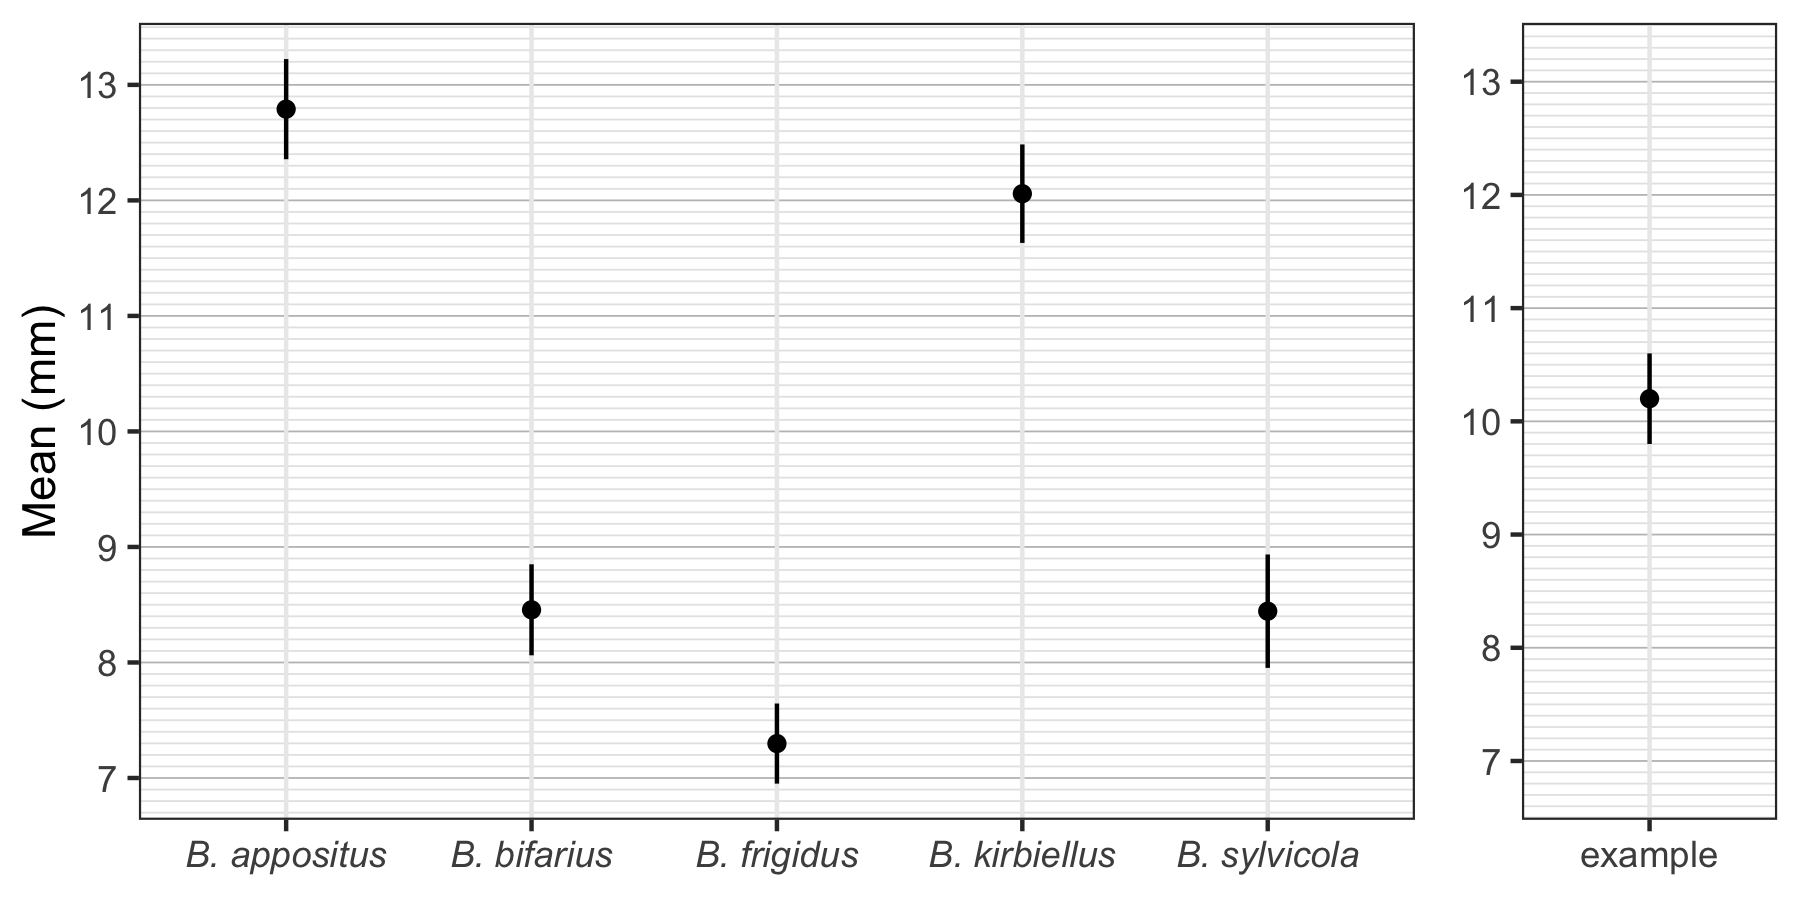
\includegraphics[width=\linewidth]{mean_proboscis_plot_key}
\else
	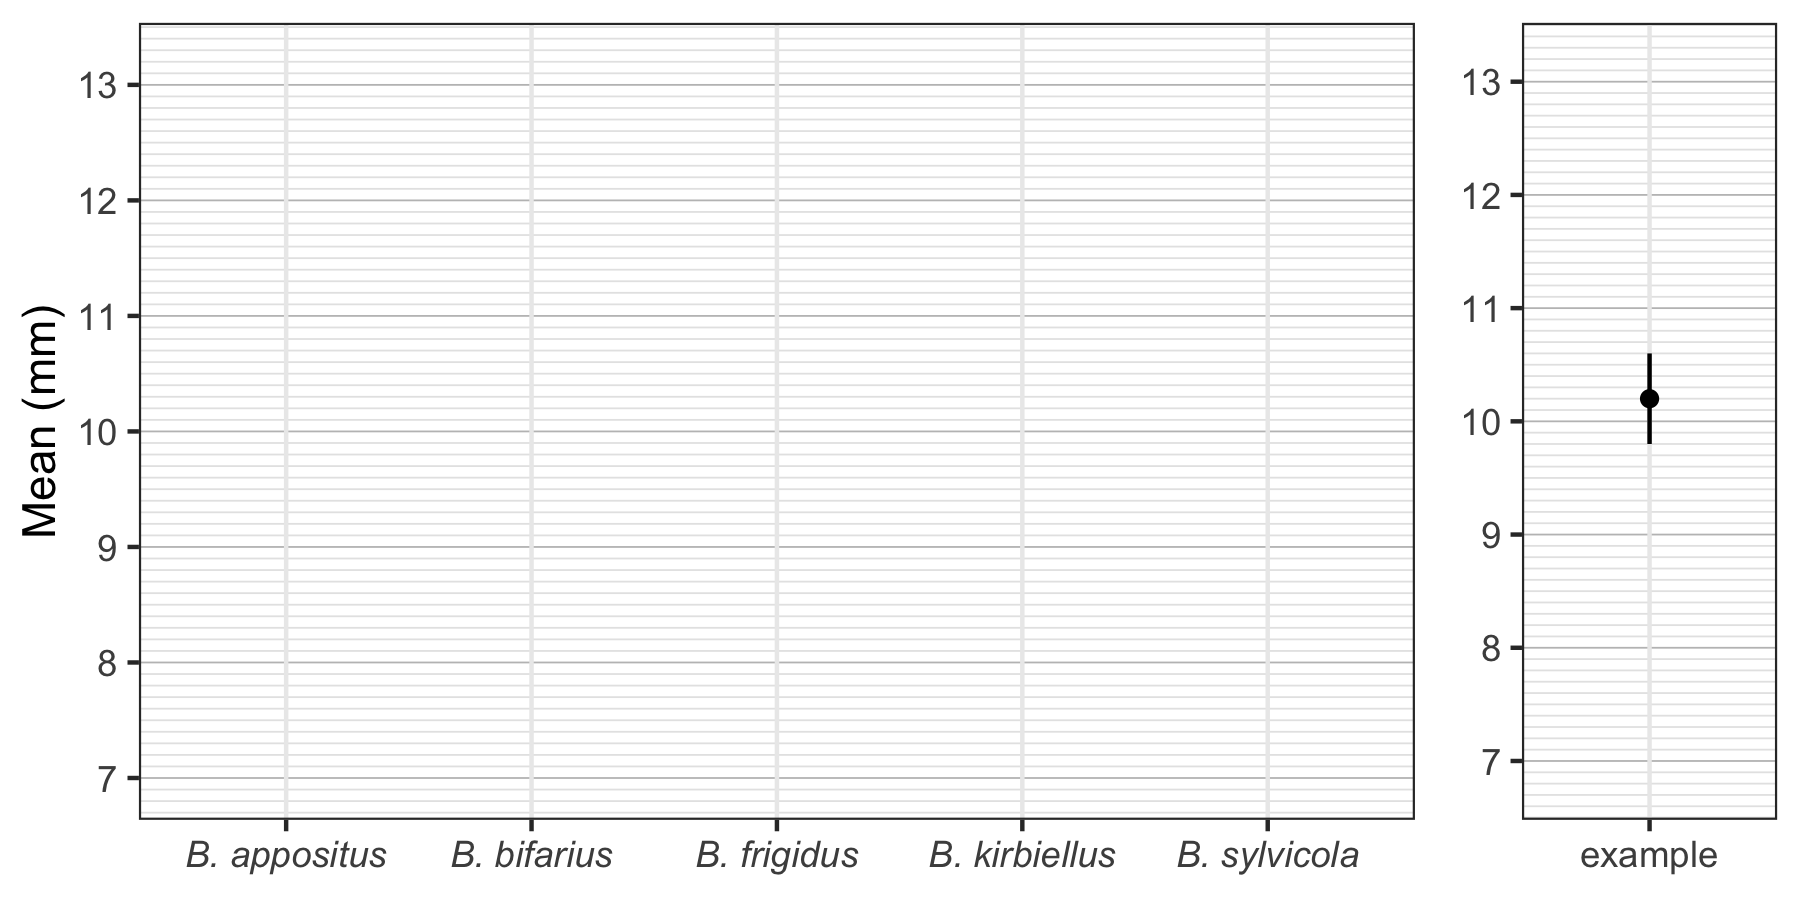
\includegraphics[width=\linewidth]{mean_proboscis_plot_blank}
\fi

%\textbf{Consider adding student-built histogram plots, or a shiny 
%	app for histograms to show spread and overlap of data.}


\question
The results suggest two size classes of \textit{Bombus}, based on
proboscis lengths.  Write the names of each species that belongs to 
each group.

\begin{tabular}{@{}ll@{}} %% ADD BLANKS for HANDOUTS.
	\toprule
	Short proboscis & Long proboscis \tabularnewline
	\midrule
	& \tabularnewline
	\ifprintanswers \textbf{\textit{B. bifarius}} \else \rule{2in}{0.4pt} \fi &
	\ifprintanswers \textbf{\textit{B. appositus}} \else \rule{2in}{0.4pt} \fi 
	\tabularnewline[2em]
	%
	\ifprintanswers \textbf{\textit{B. frigidus}} \else \rule{2in}{0.4pt} \fi &
	\ifprintanswers \textbf{\textit{B. kirbiellus}} \else \rule{2in}{0.4pt} \fi
	\tabularnewline[2em]
	%
	\ifprintanswers \textbf{\textit{B. sylvicola}} \else \rule{2in}{0.4pt} \fi &
	\rule{1in}{0.4pt} \tabularnewline
	\bottomrule
\end{tabular}

%\textbf{Consider ANOVA to test for differences in proboscis lengths. 
%	Shiny app?}

\bigskip

\question
Write a single sentence hypothesis that states how proboscis length might affect the flower size chosen by the bumble bees.

\AnswerBox{2\baselineskip}{The length of the proboscis is positively correlated with the size	of the flowers chosen by bumble bees.}

\question
Write a prediction based on your hypothesis. Remember that predictions take the form of an if\dots then statement. I'll get you started: If proboscis length determines the flower size used by a bee, then\dots

\AnswerBox{3\baselineskip}{If proboscis length determines flower size chosen, then \textit{Bombus} species with short proboscises will chose smaller flowers than species with longer proboscises.}


\subsubsection*{Analysis: proboscis length and corolla length}\label{sec:proboscis_flower_length}

Pyke et al.~(2012) measured the corolla lengths for all flowers visited by different species and castes (queens, workers, and males) of \textit{Bombus.} Their results for mean corolla and proboscis lengths are reported in the “Proboscis and corolla lengths” tab. 

\question
Make a scatterplot of the data with proboscis length on the x-axis and corolla length on the y-axis.

\ifprintanswers
	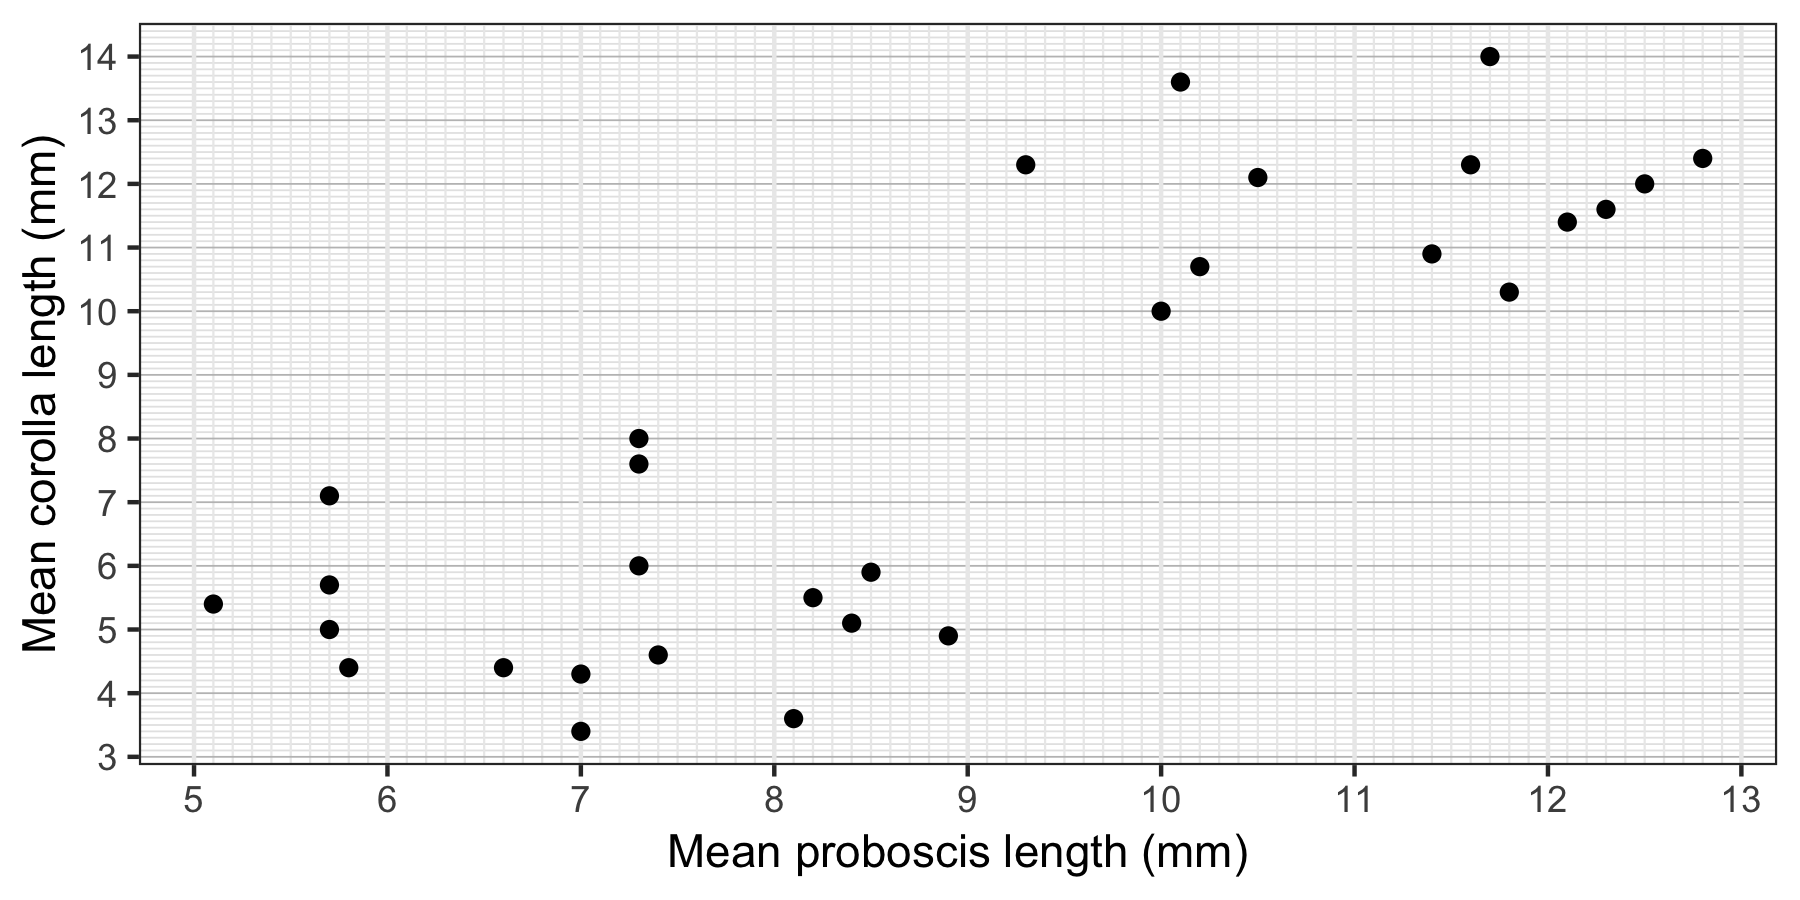
\includegraphics[width=\textwidth]{proboscis_corolla_key}
\else
	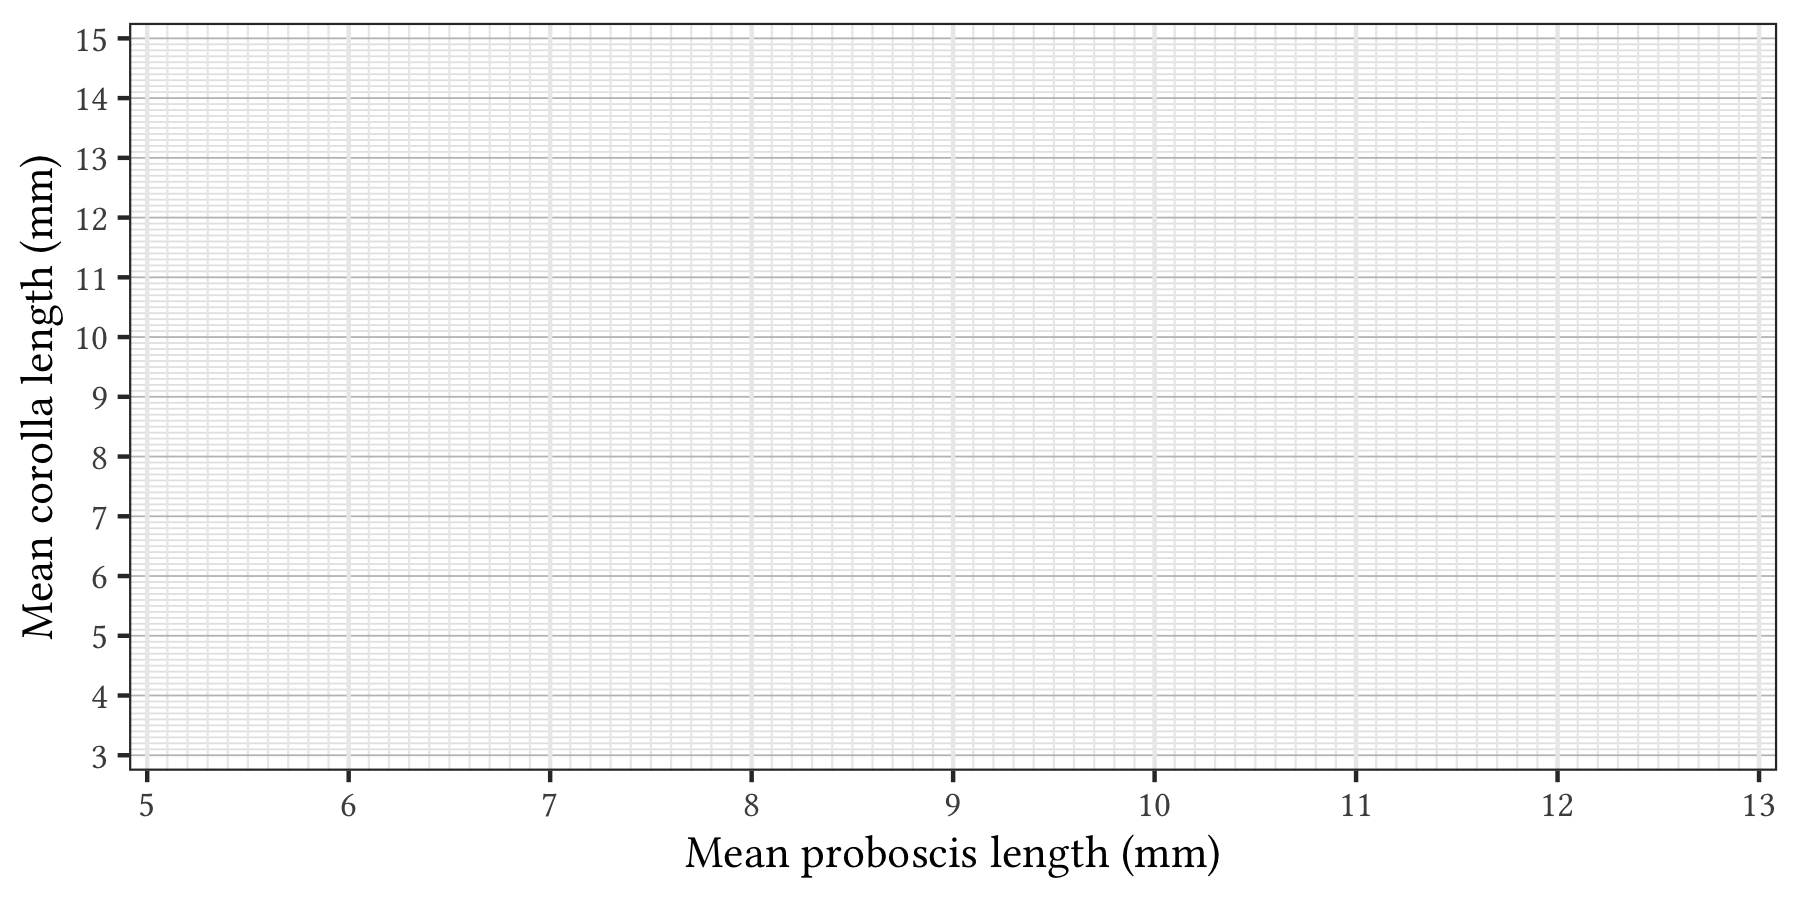
\includegraphics[width=\textwidth]{proboscis_corolla_blank}
\fi

%\textbf{Consider shiny app to do linear regression?}

\question
Do their results agree with your prediction? Explain.

\AnswerBox{0.2\textheight}{The scatterplot shows two clusters of points. 
\textit{Bombus} species with long proboscises tend to visit plant species with 
long corollas. \textit{Bombus} species with short proboscises tend to visit plant species with short corollas.}


\subsubsection*{Analysis: flower visitation by \textit{Bombus}}

The scatterplot you made was based on mean values for proboscis and corolla 
lengths. Does this show that \textit{Bombus} visited \emph{only} size-appropriate flowers?  

To answer this question Pyke (1982) recorded the flower species visited by the five \textit{Bombus} species. They recorded 7,161 visits to 34 plant species. Corolla lengths ranged from 0.0–27.2 mm. Their data are reported in the “Flower visits” tab.

To graph the data, Pyke grouped the flowers into four size classes based on corolla length. %\textbf{Make up names for size classes?}

0.00–3.99 mm\newline
4.00–7.99 mm\newline
8.00–11.99 mm\newline
12.00$+$ mm

\question
Calculate the number of visits by each species of \textit{Bombus} to each size class of flowers. %\textbf{Wording?}

\emph{Follow these instructions carefully.}

\begin{enumerate}
	\item Enter 0 mm, 4 mm, 8 mm, and 12 mm into cell row \textsc{j}1 to \textsc{m}1 (one per cell)
	to represent the \emph{minimum} corolla length needed for each size class.
	
	\item Enter the five species names into column \textsc{i}2 to \textsc{i}6.
	
	\textsc{Calculate} the number of visits by \textit{B.~appositus} to the four
	size classes of flowers. 
	
	\item Click in cell J2, and then use the \textsc{sum} function to add the
	number of flower visits in the \textit{B. appositus} column with corolla
	lengths less than 3.99~mm. For this cell, you should sum cells \textsc{c}28 to \textsc{c}35. 
	(You can sum only the cells with values, if you wish.)
	
	\item Click in cell \textsc{k}2. Sum the values for \textit{B. appositus} for
	all plant species with corolla lengths between 4.00–7.9~mm. 
	
	\item Click in cell \textsc{l}2 and sum the values for \textit{B. appositus} for
	all plant species with corolla lengths between 8.00–11.9~mm.
	
	\item Click in cell \textsc{m}2 and sum the values for \textit{B. appositus} for
	all plant species with corolla lengths 12.00~mm or longer.
	
	\item Repeat this process in the appropriate rows for the four remaining species. You can ask your instructor to check to be sure your results look correct. 
	
\end{enumerate}

\question
Use the values in your table to sketch separate column charts for the number
of visits to each size class for each species of \textit{Bombus}. Use the
blank graphs on the next page to sketch your plots.

\newpage

\ifprintanswers
	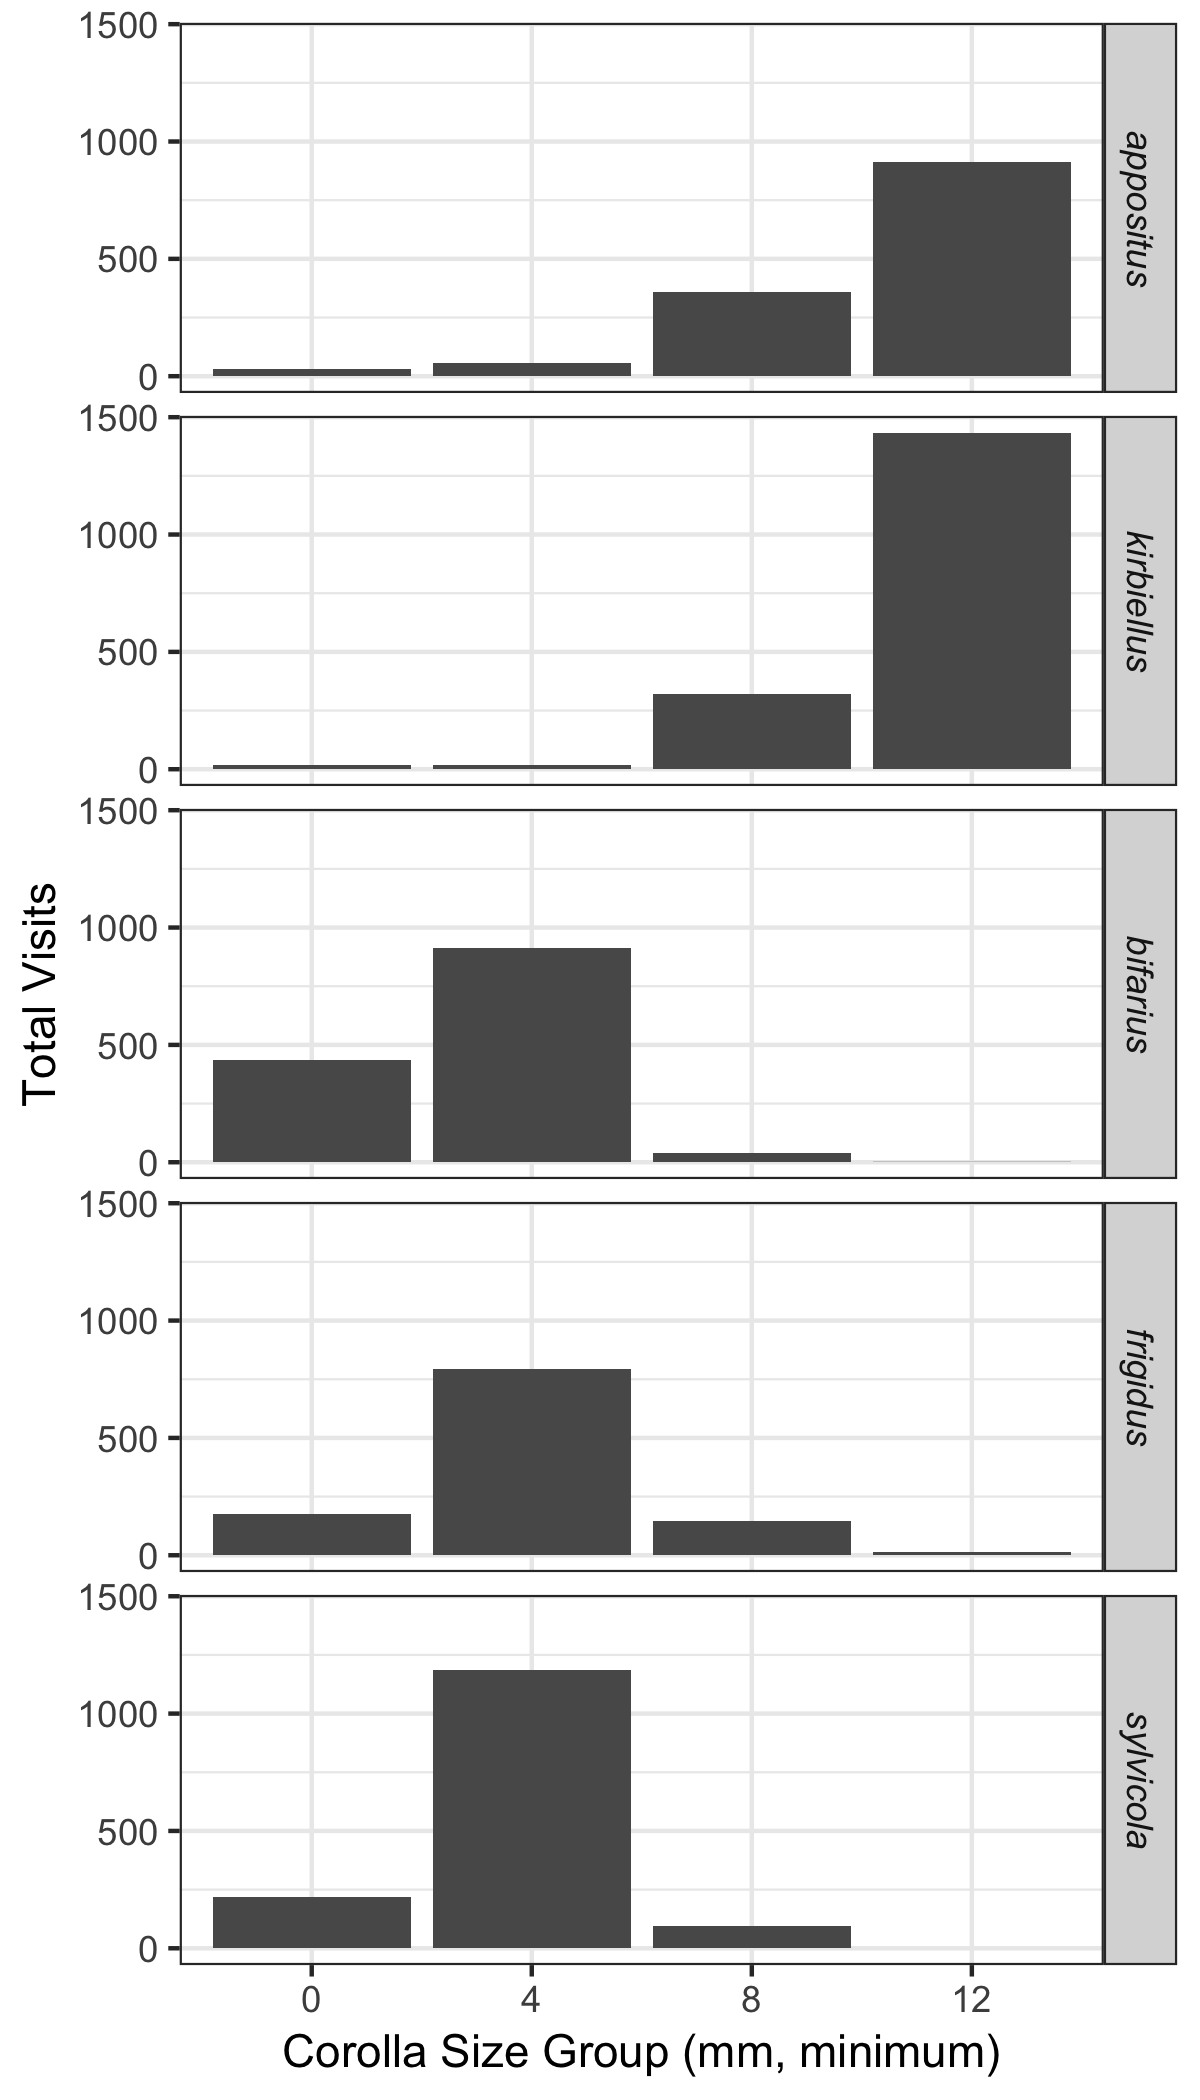
\includegraphics[height=\textheight]{flower_visits_key}
\else
	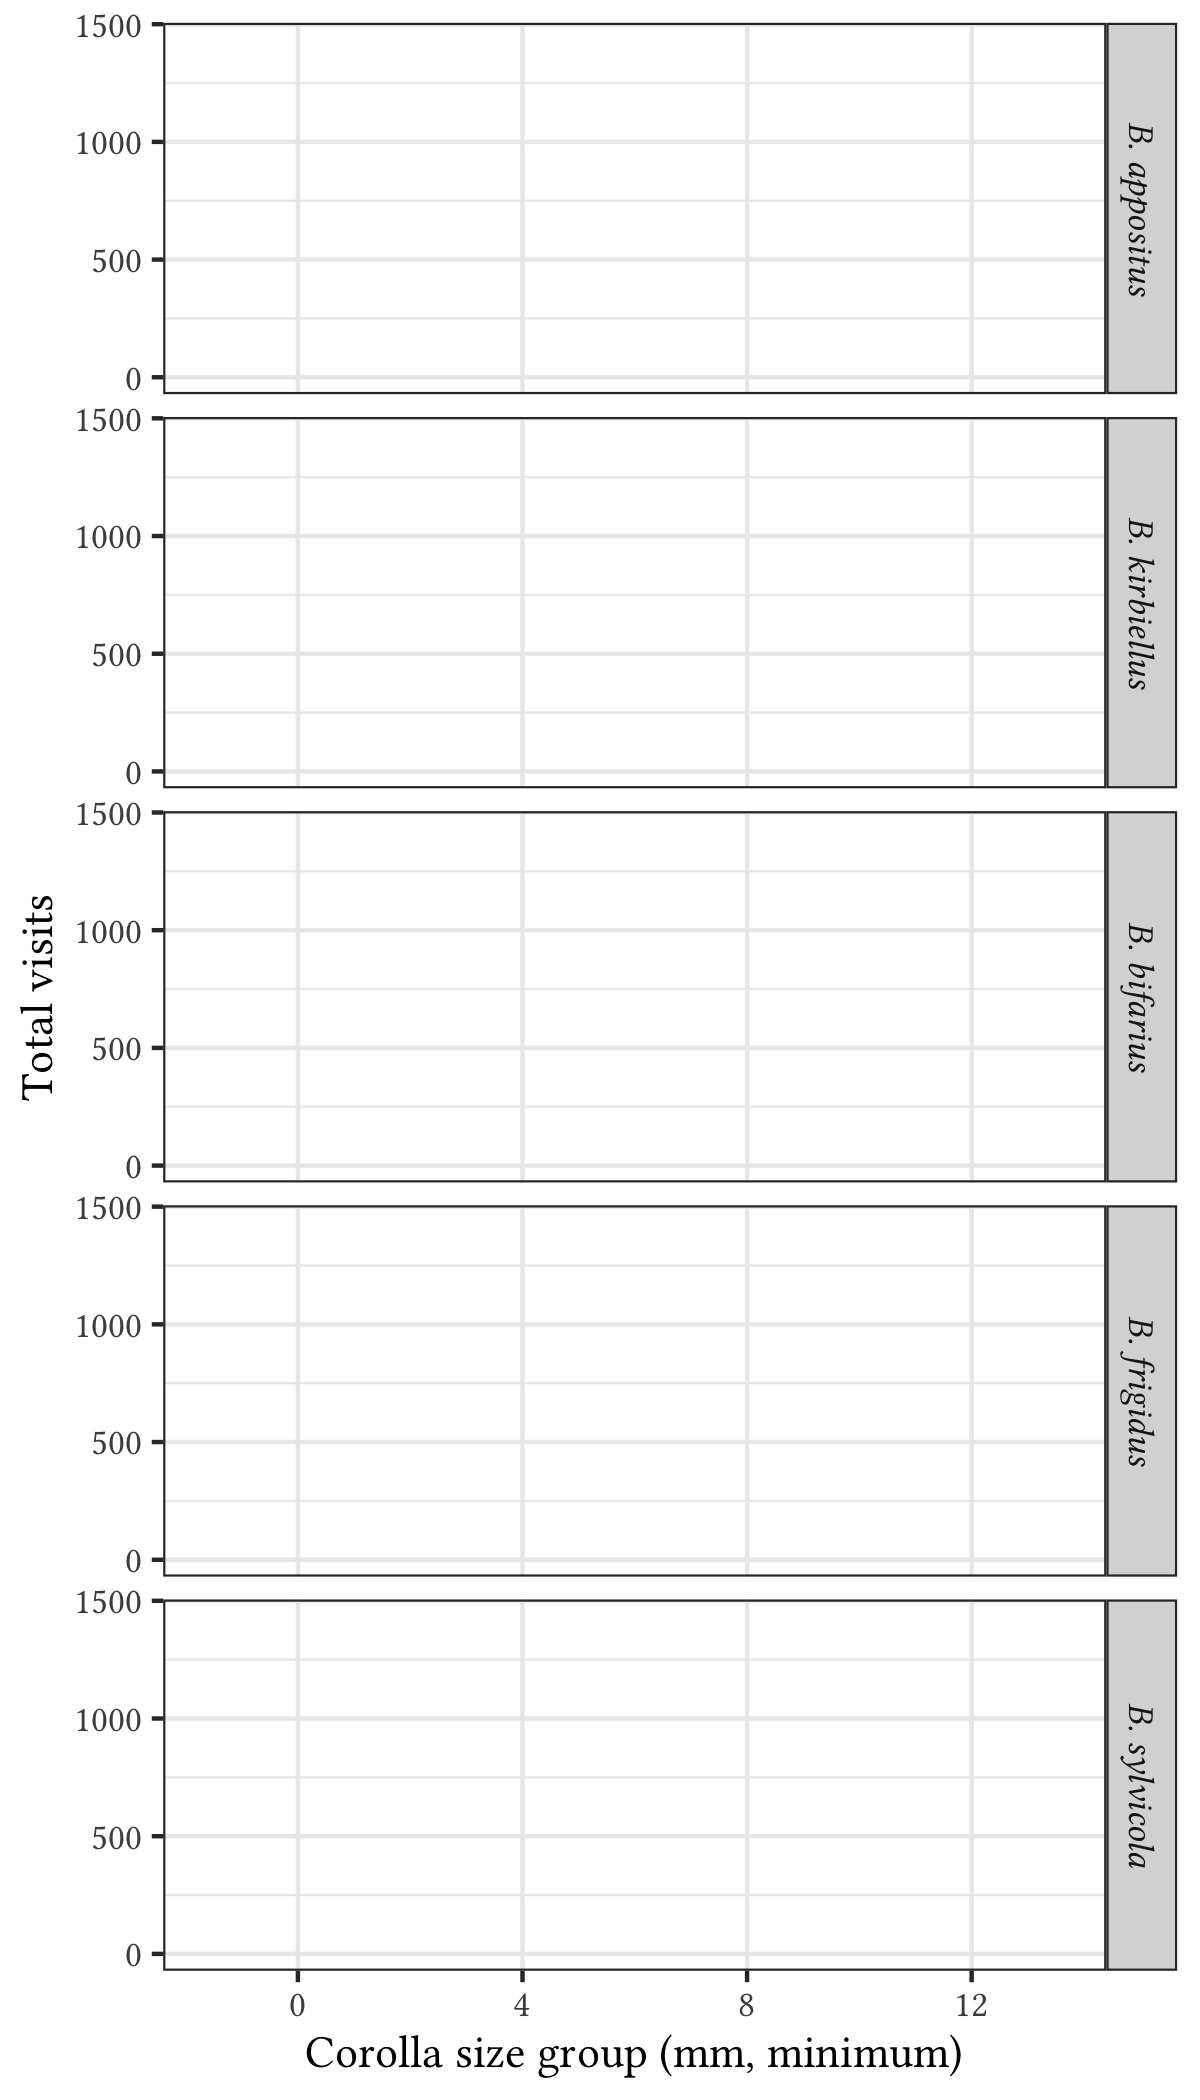
\includegraphics[height=\textheight]{flower_visits_blank}
\fi


\newpage



%\textbf{Anything about flower choice? That is more difficult to 
%tease apart but would maybe work with guidance for select plant 
%species.}


\subsubsection*{Interpret: proboscis length and flower size}

\question[Checkout]
Do the results so far provide evidence of resource partitioning?  Explain. Include all results obtained so far to support your conclusion.

\AnswerBox{0.1\textheight}{So far, the results suggest that partitioning
occurs between species with short versus long proboscises. However, bumble
bees with similar proboscis lengths use similar size flowers.}

\subsubsection*{Conclusion: proboscis length and flower size}

\question[Checkout]
Was your hypothesis supported or falsified? Explain why.

\AnswerBox{0.1\textheight}{Results support a hypothesis that at least some bumble bees partition resources based on flower size. However, those bees fall into two groups.}

\subsubsection*{Analysis: elevation and relative abundance}

Pyke (1982) noticed that the relative abundance of bees with long 
and short proboscises seemed to change as elevation increased. To 
verify his observations, Pyke calculated the relative abundance
of each species by dividing the number of individuals of
one species by the total number of individuals of all species in
the \emph{same} size class. For example, the relative abundance
of \textit{B. appositus} among long-proboscis bees was calculated by

\begin{equation*}
\dfrac{\mathrm{Number~of}~appositus}{\mathrm{Number~of}~appositus + 
\mathrm{Number~of}~kirbiellus}.
\end{equation*}

The Gothic Transect tab has the relative abundance of the five 
\textit{Bombus} species for 17 sites at elevations between 
2,873–3,697~m (9,426–12,129~ft) above sea level. The gradient becomes much steeper starting at site~11, as shown in the following table and figure.

\newpage

\begin{multicols}{2}

\begin{tabular}{@{}R{0.25in}R{0.9in}R{0.25in}R{0.9in}@{}}
	\toprule
	Site	& Elevation (m)	&	Site	&	Elevation (m) \tabularnewline
	\midrule
	1 & 2,873		& 10	& 2,985 \tabularnewline
	2 & 2,867		& 11	& 3,000 \tabularnewline
	3 & 2,885 		& 12	& 3,076 \tabularnewline
	4 & 2,915		& 13	& 3,145 \tabularnewline
	5 & 2,924		& 14	& 3,152–3,242 \tabularnewline
	6 & 2,930		& 15	& 3,242–3,333 \tabularnewline
	7 & 2,939 		& 16	& 3,333–3,485 \tabularnewline
	8 & 2,958	 	& 17	& 3,485–3,697 \tabularnewline
	9 &	2,961		&		&	\tabularnewline
	\bottomrule
\end{tabular}

\columnbreak

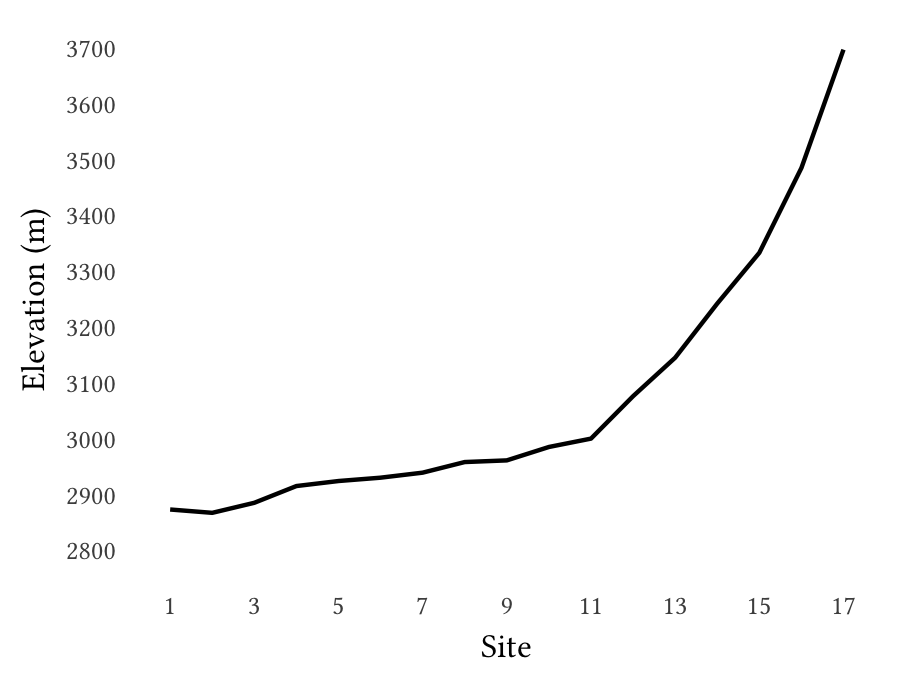
\includegraphics[width=\linewidth]{gothic_transect}

\end{multicols}

%\begin{tabular}{@{}R{0.4in}R{1in}R{0.4in}R{1in}@{}}
%	\toprule
%	\multicolumn{2}{c}{Washington Gulch} & \multicolumn{2}{c}{Schofield} \tabularnewline
%	\cmidrule(r){1-2} \cmidrule(l){3-4} 
%	Site	& Elevation (m) & Site	& Elevation (m) \tabularnewline
%	\midrule
%	1 & 2,939–3,091 	& 1	& 3,176 \tabularnewline
%	2 & 3,091–3,182 	& 2	& 3,206 \tabularnewline
%	3 & 3,182–3,242 	& 3	& 3,212–3,333 \tabularnewline
%	4 & 3,242 			& 4	& 3,333–3,485 \tabularnewline
%	5 & 3,242–3,333 	& 5	& 3,485–3,636 \tabularnewline
%	6 & 3,333 			& 6	& 3,636–3,758 \tabularnewline
%	7 & 3,333–3,394 	& 	&  \tabularnewline
%	8 & 3,394–3,442 	& 	&  \tabularnewline
%	\bottomrule
%\end{tabular}
%
\bigskip

\question
Calculate the elevation change between Site~1 and Site~11.

\AnswerBox{\baselineskip}{127~m.}

\question
Calculate the elevation change between Site~12 and Site~17 (use the 
heighest elevation for Site~17).

\AnswerBox{\baselineskip}{621~m.}

\question
Write a hypothesis that states whether species of \textit{Bombus} 
with similar proboscis lengths feed at different elevations. 

\AnswerBox{0.1\textheight}{Species with similar proboscis lengths occur at different elevations.}

\question
Turn your hypothesis into a prediction. If you were to observe bees at one site, would you predict
to see just one species of bee from the same proboscis size class? Or, might multiple
species of the same class be present but one species is much more abundant than the other species?

\AnswerBox{0.1\textheight}{If I observe bees at a single elevation, then 
I will see mostly one species of bee for a given size class.}


\question
Plot a line graph of the relative abundance of the two long-proboscis \textit{Bombus} species at each site of the Gothic Transect in the top panel of the blank graph on page~\pageref{fig:relative_abundance}. 

To make the line graph, make a dot above each site number
for the relative abundance of a species. Then connect the dots with a line. Use a solid line for \textit{B.~appositus} and a dashed 
line for \textit{B.~kirbiellus.}

\question
Plot a line graph of the relative abundance of the three 
short-proboscis \textit{Bombus} species at each site of the Gothic 
transect in the bottom panel of the blank graph on 
page~\pageref{fig:relative_abundance}. Use a solid line for 
\textit{B.~bifarius}, a short-dashed line for \textit{B.~frigidus,} 
and a long-dashed line for \textit{B.~sylvicola.}

\subsubsection*{Interpret: elevation and relative abundance}
\question
Describe how the relative abundances of \textit{B.~appositus} and 
\textit{B.~kirbiellus} change along the Gothic transect from
lower (Site~1) to higher (Site~17) elevations? At which site(s)
and elevations does one species start to become more abundant
than the other?

\AnswerBox{0.05\textheight}{\textit{B.~appositus} starts very 
high rel.~abund.~but decreases sharply between starting at
site~11. \textit{B. kirbiellus} shows the opposite pattern.}

\question
Describe how the relative abundances of \textit{B.~bifarius},
\textit{B.~frigidus}, and \textit{B.~sylvicola} change along 
the Gothic transect from lower (Site~1) to higher (Site~17) elevations? At what elevations is \textit{B.~bifarius} the
most abundant species? At what elevations is \textit{B.~frigidus} 
the most abundant species? At what elevations is \textit{B.~sylvicola} 
the most abundant species?

\AnswerBox{0.05\textheight}{\textit{B.~bifarius} is most abundant
at the lower elevation sites but is no longer the most abundant 
species by site 9–10. \textit{B.~frigidus} the most abundant species
between sites 9-11. \textit{B.~sylvicola} becomes most abundant 
between sites 12–13.}

\question
Write a statement that describes how \textit{Bombus} species with
proboscises of similar lengths partition elevation.

\AnswerBox{0.02\textheight}{Species with similar-sized proboscises
tend to occur at different elevations.}

\newpage

%\makebox[\textwidth][c]{
\label{fig:relative_abundance}
\ifprintanswers
	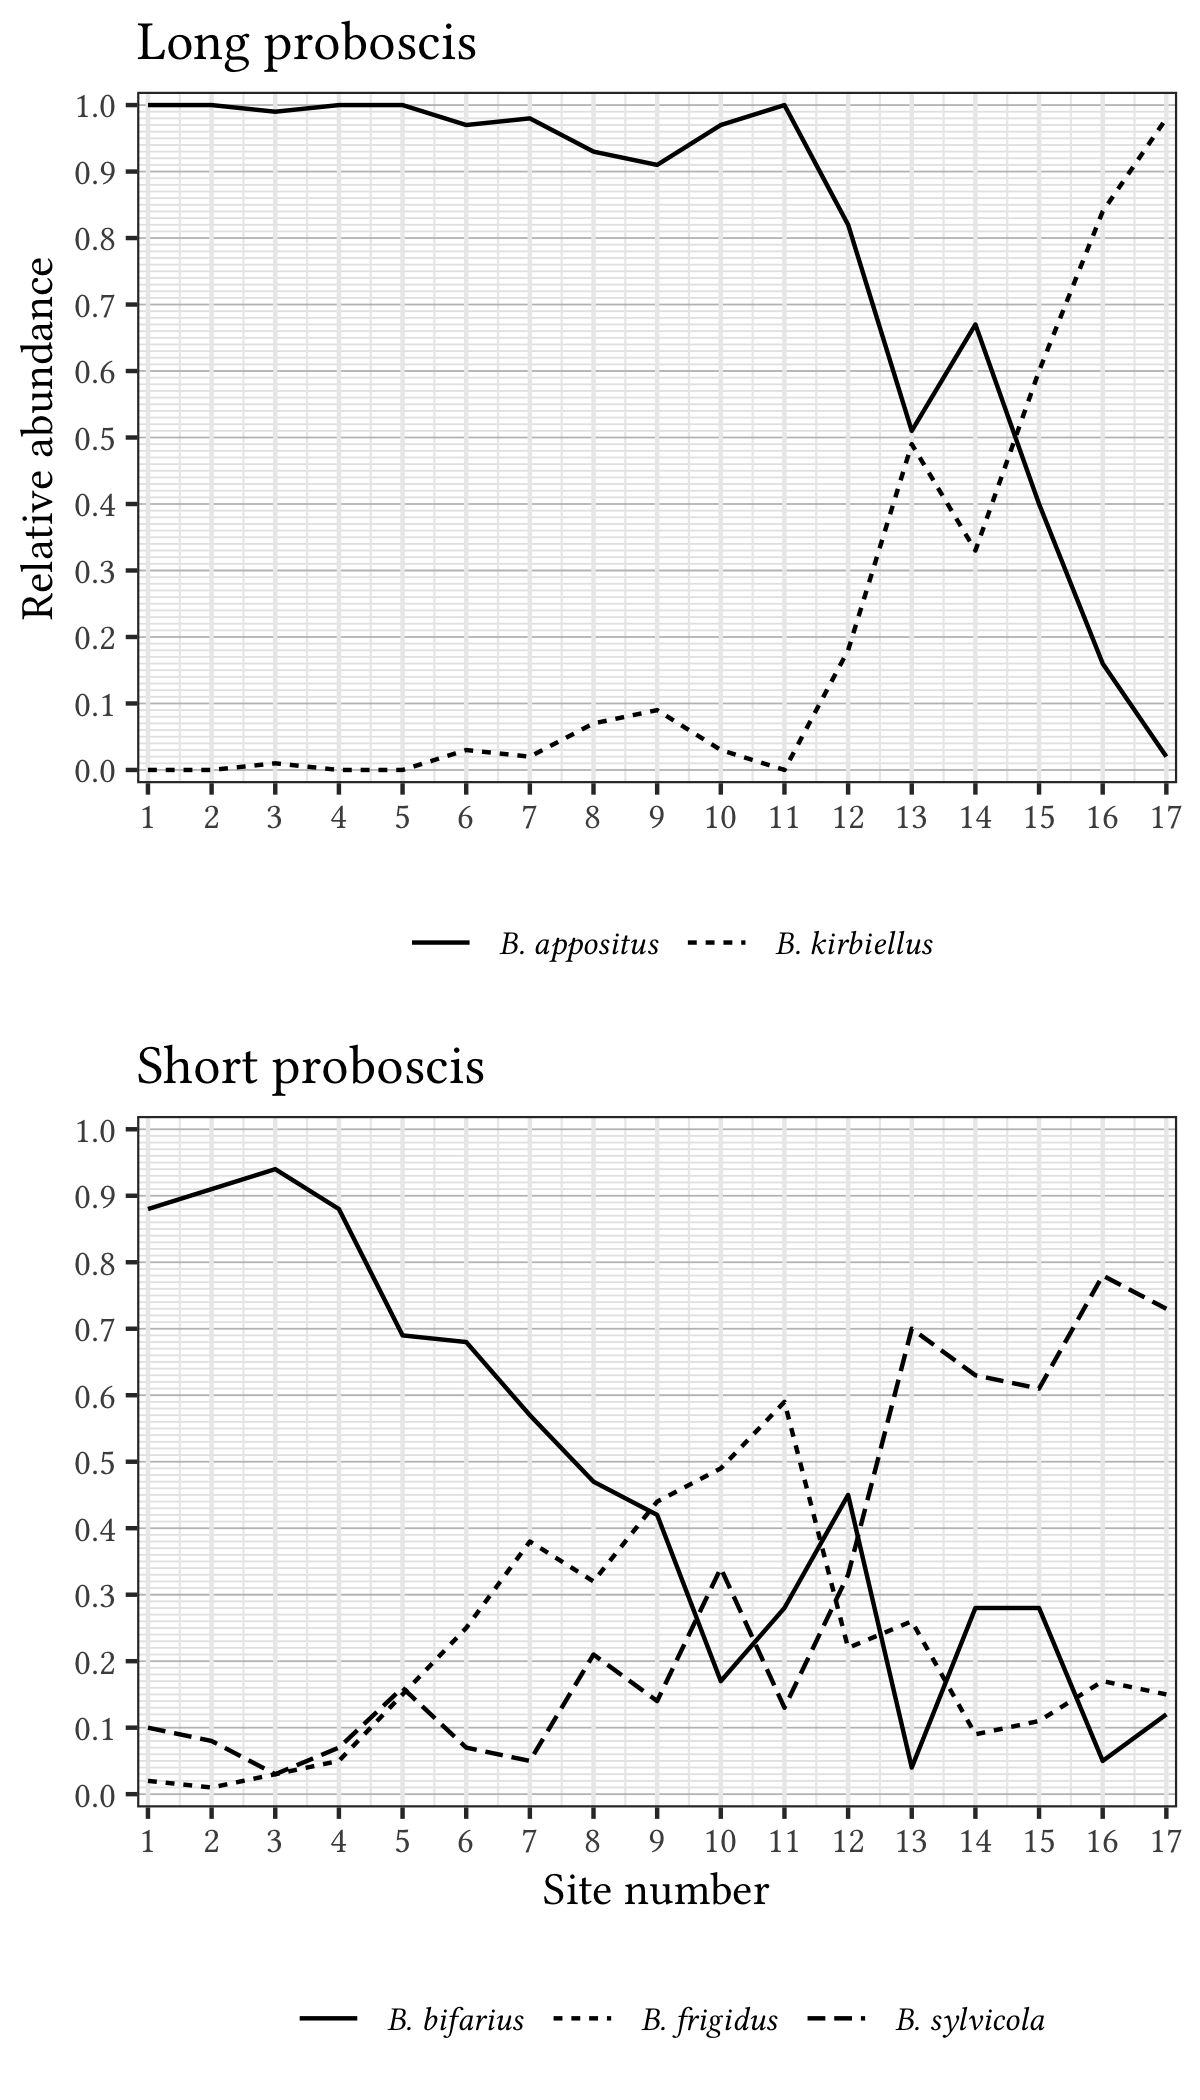
\includegraphics[height=\textheight]{gothic_relative_abundance_key}
\else
	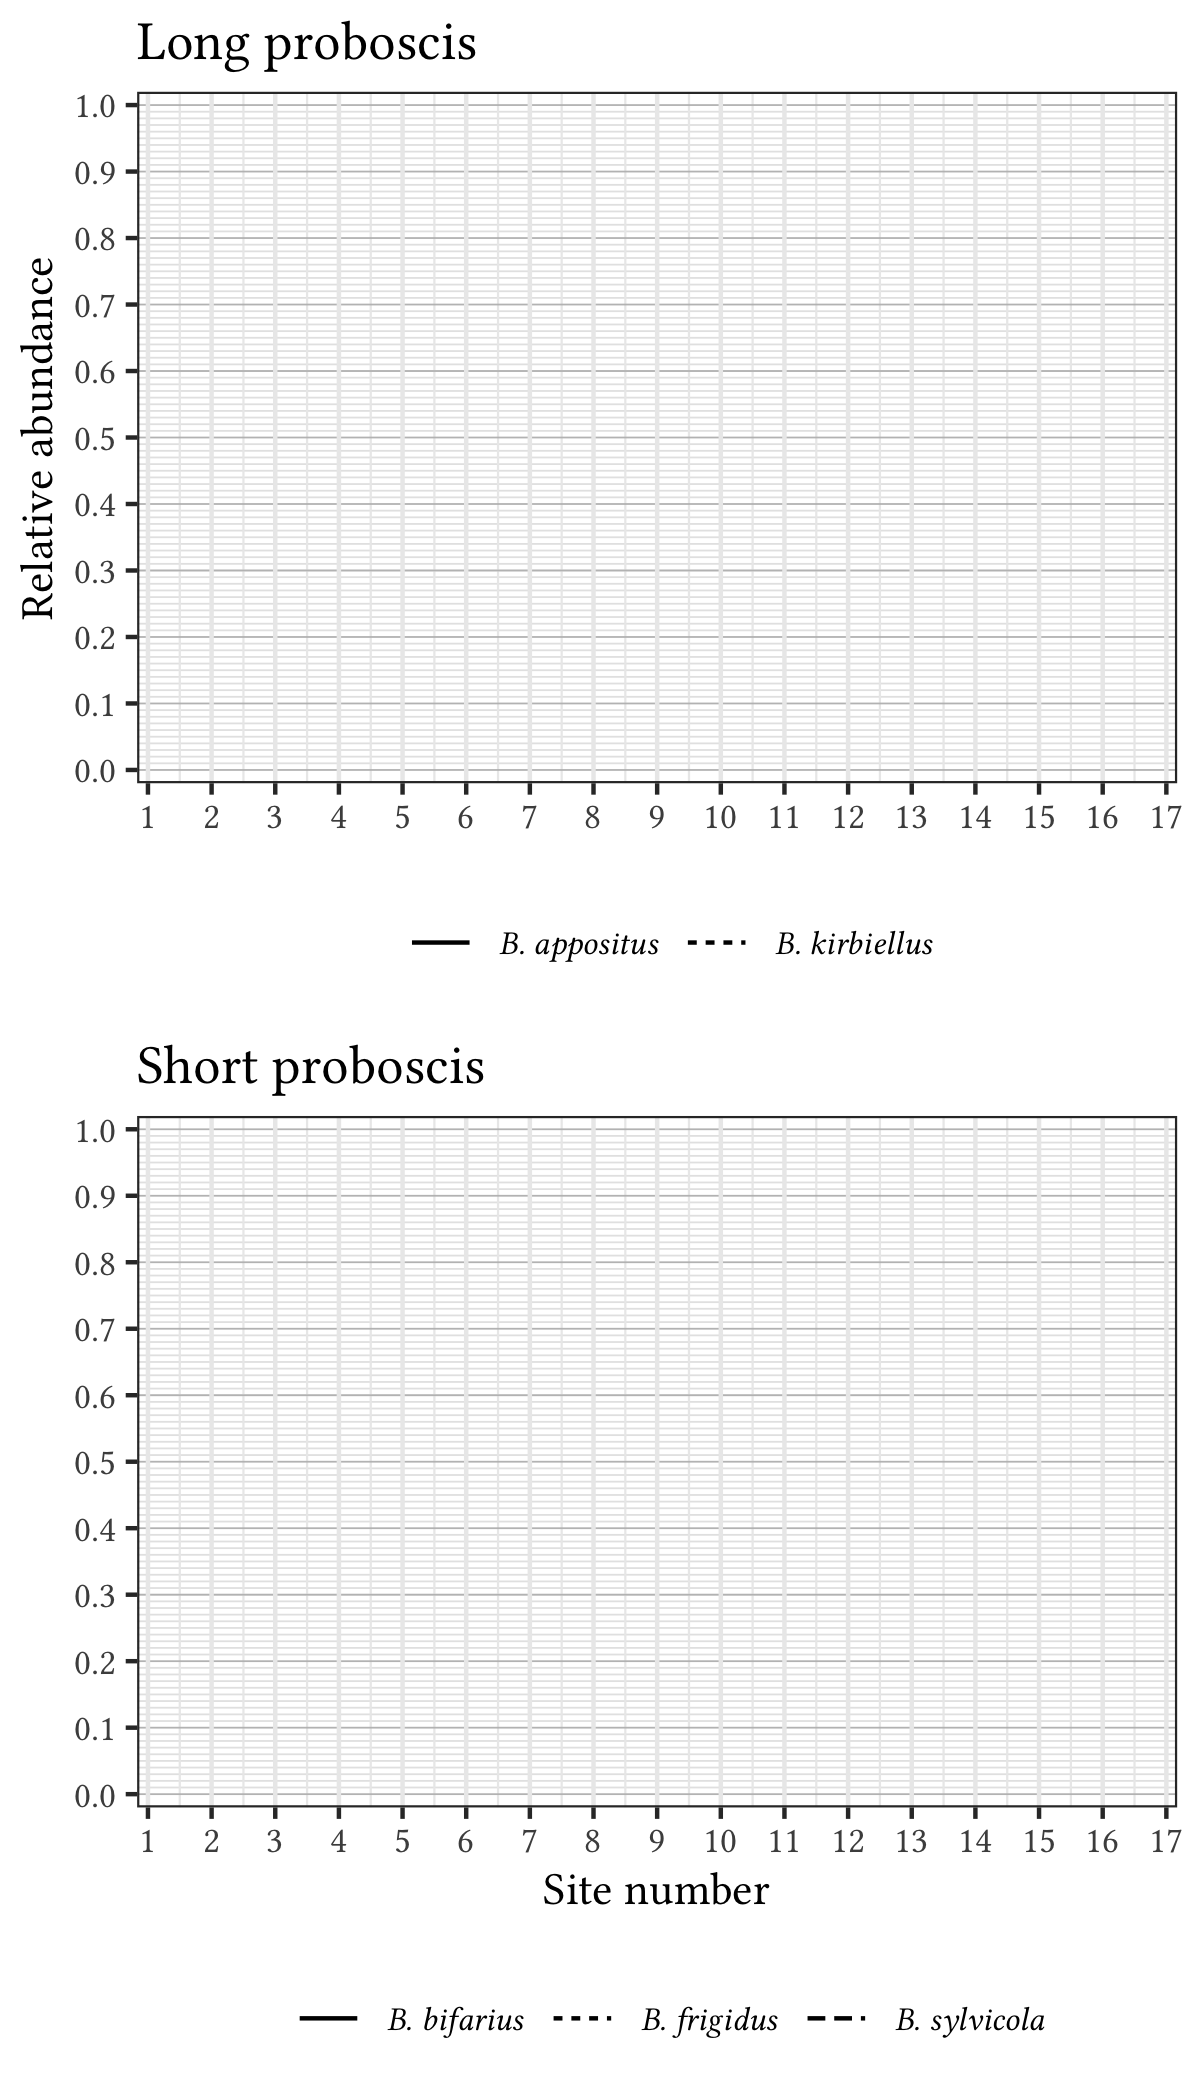
\includegraphics[height =\textheight]{gothic_relative_abundance_blank}
\fi
%}



\subsubsection*{Conclusion: resource partitioning}

\question[Checkout]
What can you conclude based on the evidence? What your hypothesis supported?

\AnswerBox{0.05\textheight}{Supported. Actually, depends on their hypothesis.}

\question[Checkout]
Describe the evidence you now have and how it supports resource partitioning of flower size and elevation among the five species of 
\textit{Bombus} bumble bees studied here.


\begin{AnswerPage}{0.2\textheight}
The five species of \textit{Bombus} bumble bees partition their
nectar sources based on the length of their proboscises. Species
with shorter proboscises visit smaller flowers more often and 
vice versa for species with long proboscises.

Species with similar lengths of proboscises tend to partition
elevation. At with one species usually dominant at a similar 
elevations. As elevation increases, another species tends to become
more abundant.
\end{AnswerPage}


\end{questions}


\subsubsection*{Literature Cited}

\begin{hangparas}{\leftmargin}{1}

Macior, L.\,W. 1974. Pollination ecology of the front
range of the Colorado Rocky Mountains. Melanderia 15: 1–59.

Pyke, G.\,H. 1982. Local geographic distributions of bumblebees 
near Crested Butte, Colorado: competition and community structure.
Ecology 63: 555–573.

Pyke, G.\,H., D.\,W.\,Inouye, and J.\,D.\,Thomson. 2012. Local geographic distributions of bumble bees near Crested Butte, Colorado: competition and community structure revisited. Environmental Entomology 41: 1332–1349.

\end{hangparas}

\end{document}  